\documentclass{article}
\usepackage{graphicx}
\usepackage{amsmath}
\usepackage{tikz}
\usepackage{soul}
\usepackage[colorinlistoftodos]{todonotes}
\usepackage{booktabs}
\usepackage{array}
\usepackage{float}
\usepackage{algorithm}
\usepackage{algpseudocode}
\usepackage{geometry}  % Added for better margin handling
\usepackage{multirow}  % For the class distribution table
\usepackage{caption}   % For better caption handling
\usepackage{siunitx}   % For better number formatting
% hyperref for references
\usepackage{hyperref}
\usepackage{graphicx}
\usepackage{multirow}
\usepackage{booktabs}
\usepackage{pgfplots}
\pgfplotsset{compat=1.18}
\usepackage{multirow}
\usepackage{booktabs}
\usepackage{makecell}

% Set more generous margins
\geometry{
    margin=1in
}

\usetikzlibrary{shapes,arrows,positioning,calc}

\title{CPET Analysis}
\author{Aaron HA Fletcher}
\date{September 2024}

\begin{document}
\maketitle

\section{Non-time-series data}
\subsection{Preprocessing and Dimensionality Reduction}
Input data was matched to the output data by research ID. All inputs and outputs were checked to ensure that no duplicates were present. If duplicates were present, and they were identical duplications, only one of the duplicates was kept. There were 4 cases of duplicates in the output data on Research ID, where the row with the complete information was selected (index 2010, 2167, 2287, 2742).

Data was valid if it had a corresponding valid BxB file. A valid BxB file is one which has more than 100 lines of data.
This resulted in 3892 valid input and output records, with 256 features. All categorical features were label encoded.

Engineered features were calculated from the DateOfCPETtest and OperationDate. Each test was validated as a date (format MM/DD/YYYY, a valid calendar date and checked to ensure year was not before 1900 and after 2024). Each date was then represented as cyclical encoding using sin/cos functions, extracted to year, month and day, represented as day of the week, day of the month, boolean weekend indicator and year quarter.

Missing values were imputed using the mean of that feature. Any features that needed 30\% or more of their values imputed were removed. This resulted in the removal of 17 features in table \ref{tab:missing-values}. Counts of missing values by remaining features are in table \ref{tab:imputation-summary}.

Finally this 259 dimensional dataset was reduced to 90\% explained variance using PCA. 97 features were dropped based on features with a PCA-importance score based on PCA loadings being below mean - standard deviation or correlation coefficient being above 0.9. The features dropped within this approach are listed in table \ref{tab:features-to-remove}. The final dataset had the shape (3892, 162).

% Fixed the overfull line by breaking it into multiple lines
The binary outcome labels were switched for:
\begin{itemize}
    \item Days\_at\_home\_90\_days\_Binary
    \item Days\_at\_home\_180\_days\_Binary
\end{itemize}
This was done as the minority class was originally 0.

\subsection{Dataset characteristics}

The dataset was split using a stratified approach to ensure balanced representation of all six binary outcomes across the splits. First, the data was divided into 80\% training+validation and 20\% testing sets. The 80\% portion was further split into 81.25\% training and 18.75\% validation, resulting in final proportions of 65\% training, 15\% validation, and 20\% testing of the total dataset. This yielded 2,529 training examples, 584 validation examples, and 779 testing examples.
To maintain the distribution of all binary outcomes (90-day and 180-day days at home, and 30-day, 90-day, 720-day, and 1,825-day mortality), a composite stratification variable was created by combining all six outcomes. For example, a patient with positive 90-day days at home, negative 180-day days at home, and negative mortality outcomes would be assigned to the stratum ''1\_0\_0\_0\_0\_0". This approach ensured that the relative proportions of all possible outcome combinations remained consistent across the splits.
The class distributions for each outcome are shown in Table 1, where class 1 represents the minority class and class of interest (positive class) for each outcome. The stratified splitting successfully maintained similar class distributions across all splits, with the most imbalanced being 30-day mortality (2.3\% positive cases) and the most balanced being 1,825-day mortality (23.2\% positive cases).
Class distribution is in table \ref{tab:class-distribution}, with class 1 being the minority class and the class of interest (positive class). Due to the extreme class imbalance, SMOTE was not used as it would have resulted in more synthetic samples than actual positive cases.

\subsection {Evaluation metrics}

Precision-Recall AUC was used to evaluate the performance of models during hyperparameter tuning. Precision is the ratio of tp / (tp + fp) where tp is the number of true positives and fp is the number of false positives. Recall is the ratio of tp / (tp + fn) where tp is the number of true positives and fn is the number of false negatives. Precision-recall is calculated at different probability thresholds, based on every unique probability score in validation set. Area under the curve is then used to evaluate the overall performance of the model. PR AUC is used because the dataset is highly imbalanced, and precision and recall are more important than accuracy. PR AUC is also used over ROC AUC as it is more sensitive to the performance of the minority class.


\subsection{Model hyperparameter tuning}

A variety of models were explored for the non-time series data, such as linear models (Logistic Regression, Support Vector Machines), Tree-based models (Random Forest), Neural Netowrks (Deep Neural Networks), Probabalistic Models (Maximum Entropy) and instance based models (K-Nearest Neighbours).
For each model, a hyperparameter grid search was performed using the training and validation sets to find the best performing hyperparameters. The hyperparameter search space is outlined for each model in table \ref{tab:hyperparameters}. Successful models were those which had the greatest Precision-Recall AUC score on the validation set and predicted the positive class. Final model hyperparameters are shown in table \ref{tab:final-model-hyperparameters} along with their PR AUC score on the test set.

\subsubsection{Model specific adjustments}

Owing to the extreme class imbalance, adjustments were made to some models to improve their PR AUC score.
\begin{itemize}
    \item Grid search was performed using class weights. Class weights are used to balance the loss / cost function for the minority class during training.
    \item DNN were trained using focal loss. Focal loss is used to prevent the model from being overconfident on the majority class.
    \item DNN used dropout to prevent overfitting on the majority class.
    \item KNN used sample replication to balance the class distribution based on class\_weight function.
    \item Class weighting was used for all models.
    \item Models predictions were performed using an optimum threshold as derived from validation data split, to reduce overly aggressive or conservative predictions.
\end{itemize}

\subsection{Grid search results}

Best models were selected based on dual criteria: Predicted at least 1\% of the positive class and Highest PR AUC score on the validation set. Outcome model specific hyperparameter tuning results on the validation set are in table \ref{tab:final-model-hyperparameters}. Generally, DNN models performed best in all cases with PR AUC scores, except for 30 day mortality, where KNN performed best. I expect that this is due to the extreme class imbalance within the Mortality at 30 days outcome (2.3\% positive cases).

\subsection{Test set performance}




\begin{table}[H]
    \centering
    \begin{tabular}{lr}
        \toprule
        \textbf{Feature}        & \textbf{Missing (\%)} \\
        \midrule
        Haematocrit             & 96.4                  \\
        MeanCellHaemoglobinConc & 59.6                  \\
        Neutrophilsx109L        & 99.8                  \\
        Lymphocytesx109L        & 99.8                  \\
        Monocytesx109L          & 99.8                  \\
        Eosinophilsx109L        & 99.8                  \\
        Basophilsx109L          & 99.9                  \\
        TotalProteingL          & 30.7                  \\
        Globulin                & 100.0                 \\
        TotalbilirubinumolL     & 31.6                  \\
        AlkalinephosphataseIUL  & 31.0                  \\
        ALTUL                   & 31.2                  \\
        ASTUL                   & 99.8                  \\
        CalciummmolL            & 35.1                  \\
        AdjustedcalciummmolL    & 36.3                  \\
        CRPmgL                  & 65.1                  \\
        FerritinugL             & 62.6                  \\
        \bottomrule
    \end{tabular}
    \caption{Percentage of Missing Values by Features}
    \label{tab:missing-values}
\end{table}


\begin{table}[H]
    \centering
    \small
    \begin{tabular}{lrr}
        \toprule
        \textbf{Feature}              & \textbf{Missing Values} & \textbf{Mean Value Used} \\
        \midrule
        VO2\_mLminmLmin@Rest          & 145                     & 393.41                   \\
        VO2\_mLminmLmin@WorkMax       & 25                      & 1219.43                  \\
        VO2\_mLminmLmin@MaxValue      & 25                      & 1520.11                  \\
        VO2\_mLminmLmin@VO2MaxPred    & 25                      & 84.86                    \\
        VO2\_mLminmLmin@WorkMaxPred   & 25                      & 71.92                    \\
        VO2\_mLminmLmin@ATVO2Max      & 70                      & 70.45                    \\
        VO2\_mLminmLmin@ATPred        & 70                      & 57.17                    \\
        VO2\_mLminmLmin@ATWorkMax     & 70                      & 84.05                    \\
        Work\_WattsWatts@PredMax      & 58                      & 115.38                   \\
        Work\_WattsWatts@AT           & 339                     & 55.51                    \\
        Work\_WattsWatts@VO2Max       & 252                     & 80.18                    \\
        Work\_WattsWatts@WorkMax      & 64                      & 86.16                    \\
        Work\_WattsWatts@MaxValue     & 64                      & 86.16                    \\
        Work\_WattsWatts@VO2MaxPred   & 280                     & 74.13                    \\
        Work\_WattsWatts@ATVO2Max     & 468                     & 92.09                    \\
        Work\_WattsWatts@ATPred       & 370                     & 51.25                    \\
        Work\_WattsWatts@ATWorkMax    & 339                     & 62.33                    \\
        VO2WorkSlopemLminwatt@AT      & 621                     & 8.99                     \\
        VO2WorkSlopemLminwatt@VO2Max  & 471                     & 15.01                    \\
        VO2WorkSlopemLminwatt@WorkMax & 347                     & 8.10                     \\
        MeanCellVolumefL              & 560                     & 87.66                    \\
        HaemoglobingL                 & 555                     & 129.63                   \\
        Whitecellcountx109L           & 555                     & 7.94                     \\
        Plateletsx109L                & 561                     & 267.02                   \\
        RBCcountx1012L                & 560                     & 4.44                     \\
        SodiummmolL                   & 530                     & 138.89                   \\
        PotassiummmolL                & 547                     & 4.37                     \\
        UreammolL                     & 515                     & 6.16                     \\
        CreatinineumolL               & 513                     & 87.74                    \\
        eGFR\_Calculated              & 516                     & 77.54                    \\
        AlbumingL                     & 733                     & 41.45                    \\
        Age                           & 9                       & 70.66                    \\
        Sex                           & 3                       & 1.37                     \\
        Height                        & 4                       & 168.72                   \\
        Weight                        & 3                       & 80.66                    \\
        NewBMI                        & 4                       & 28.24                    \\
        IMD\_SCORE                    & 10                      & 7.30                     \\
        LeesCRIfactors                & 336                     & 0.34                     \\
        TotalPolyPharm                & 336                     & 2.06                     \\
        PolyPharm\_Cat                & 336                     & 1.11                     \\
        \bottomrule
    \end{tabular}
    \caption{Summary of Feature Imputation}
    \label{tab:imputation-summary}
\end{table}


\begin{table}[ht]  % Changed from [h] to [ht]
    \centering
    \begin{tabular}{|l|}
        \hline
        \textbf{Feature Name}           \\
        \hline
        ChronotropicIndex               \\
        DateofCPETtest\_day\_cos        \\
        DateofCPETtest\_day\_sin        \\
        DateofCPETtest\_is\_weekend     \\
        DateofCPETtest\_month\_cos      \\
        DateofCPETtest\_month\_sin      \\
        DateofCPETtest\_quarter\_cos    \\
        DateofCPETtest\_quarter\_sin    \\
        HRR@AT                          \\
        HRR@ATVO2Max                    \\
        HRR@MaxValue                    \\
        HRR@Rest                        \\
        Operationdate\_day\_cos         \\
        Operationdate\_day\_sin         \\
        Operationdate\_is\_weekend      \\
        Operationdate\_month\_cos       \\
        Operationdate\_month\_sin       \\
        Operationdate\_quarter\_cos     \\
        Operationdate\_quarter\_sin     \\
        Systemicsteroid                 \\
        VCO2\_mLminmLmin@ATPred         \\
        VCO2\_mLminmLmin@VO2MaxPred     \\
        VCO2\_mLminmLmin@WorkMaxPred    \\
        VEVCO2@ATPred                   \\
        VEVCO2@VO2MaxPred               \\
        VEVCO2@WorkMaxPred              \\
        VEVO2@ATPred                    \\
        VEVO2@VO2MaxPred                \\
        VEVO2@WorkMaxPred               \\
        VdVt\_est@ATWorkMax             \\
        VO2HRmLbeat@ATPred              \\
        VO2HRmLbeat@VO2MaxPred          \\
        VO2HRmLbeat@WorkMaxPred         \\
        VO2Pred@AT                      \\
        VO2Pred@MaxValue                \\
        VO2Pred@Rest                    \\
        VO2Pred@VO2Max                  \\
        VO2Pred@WorkMax                 \\
        VO2WorkSlopemLminwatt@AT        \\
        VO2WorkSlopemLminwatt@ATVO2Max  \\
        VO2WorkSlopemLminwatt@ATWorkMax \\
        VO2\_kgmLkgmin@ATPred           \\
        VO2\_kgmLkgmin@VO2MaxPred       \\
        VO2\_kgmLkgmin@WorkMaxPred      \\
        VO2\_mLminmLmin@ATPred          \\
        VO2\_mLminmLmin@VO2MaxPred      \\
        VO2\_mLminmLmin@WorkMaxPred     \\
        \hline
    \end{tabular}
    \caption{List of Features Selected for Removal}
    \label{tab:features-to-remove}
\end{table}

\begin{table}[H]
    \centering
    \begin{tabular}{l|rr|rr|rr|rr}
        \toprule
        \multirow{2}{*}{\textbf{Outcome}} & \multicolumn{2}{c|}{\textbf{All Data}} & \multicolumn{2}{c|}{\textbf{Train Set}} & \multicolumn{2}{c|}{\textbf{Validation Set}} & \multicolumn{2}{c}{\textbf{Test Set}}                                                                             \\
        \cmidrule(lr){2-3} \cmidrule(lr){4-5} \cmidrule(lr){6-7} \cmidrule(lr){8-9}
                                          & \textbf{Class 0}                       & \textbf{Class 1}                        & \textbf{Class 0}                             & \textbf{Class 1}                      & \textbf{Class 0} & \textbf{Class 1} & \textbf{Class 0} & \textbf{Class 1} \\
        \midrule
        Days at home (90 days)            & 91.3\%                                 & 8.7\%                                   & 2310                                         & 219                                   & 533              & 51               & 712              & 67               \\
        Days at home (180 days)           & 94.1\%                                 & 5.9\%                                   & 2382                                         & 147                                   & 549              & 35               & 733              & 46               \\
        Mortality (30 days)               & 97.7\%                                 & 2.3\%                                   & 2471                                         & 58                                    & 570              & 14               & 761              & 18               \\
        Mortality (90 days)               & 97.1\%                                 & 2.9\%                                   & 2456                                         & 73                                    & 567              & 17               & 757              & 22               \\
        Mortality (720 days)              & 88.4\%                                 & 11.6\%                                  & 2235                                         & 294                                   & 516              & 68               & 689              & 90               \\
        Mortality (1825 days)             & 76.8\%                                 & 23.2\%                                  & 1943                                         & 586                                   & 449              & 135              & 599              & 180              \\
        \bottomrule
    \end{tabular}
    \caption{Class distribution across all data splits}
    \label{tab:class-distribution}
\end{table}

\begin{table}[htbp]
    \centering
    \caption{Hyperparameter Search Space for All Models}
    \begin{tabular}{llll}
        \toprule
        \textbf{Model}              & \textbf{Hyperparameter} & \textbf{Values}                                & \textbf{Description}     \\
        \midrule
        \multirow{7}{*}{DNN}        & Layer Sizes             & \{(32), (64), (128),                           & Number and size of       \\
                                    &                         & (64, 32), (128, 64),                           & hidden layers            \\
                                    &                         & (256, 128)\}                                   &                          \\
                                    & Activation              & \{relu, tanh, elu\}                            & Activation function      \\
                                    & Dropout Rate            & \{0.0, 0.2\}                                   & Regularization strength  \\
                                    & Optimizer               & \{adam, sgd\}                                  & Optimization algorithm   \\
                                    & Learning Rate           & \{0.001, 0.01\}                                & Step size                \\
                                    & Batch Size              & \{32, 64\}                                     & Mini-batch size          \\
                                    & Epochs                  & \{10, 20, 30, 50\}                             & Training iterations      \\
        \midrule
        \multirow{5}{*}{KNN}        & n\_neighbors            & \{3, 5, 7, 9, 11\}                             & Number of neighbors      \\
                                    & weights                 & \{uniform, distance\}                          & Weight function          \\
                                    & metric                  & \{euclidean, manhattan\}                       & Distance metric          \\
                                    & class\_weight           & \{None, balanced, \{0:1, 1:10/25/50\}\}        & Class weighting scheme   \\
                                    & leaf\_size              & \{30, 60, 90\}                                 & Leaf size for tree       \\
        \midrule
        \multirow{6}{*}{Logistic}   & C                       & \{0.001, 0.01, 0.1, 1.0,                       & Inverse of               \\
        \multirow{6}{*}{Regression} &                         & 10.0, 100.0\}                                  & regularization strength  \\
                                    & penalty                 & \{l1, l2, elasticnet\}                         & Regularization type      \\
                                    & solver                  & \{liblinear, saga,                             & Optimization algorithm   \\
                                    &                         & newton-cg, lbfgs\}                             &                          \\
                                    & class\_weight           & \{None, balanced,                              & Class weighting scheme   \\
                                    &                         & \{0:1, 1:10/25/50\}\}                          & for imbalanced data      \\
        \midrule
        \multirow{6}{*}{Random}     & n\_estimators           & \{100, 200, 500\}                              & Number of trees          \\
        \multirow{6}{*}{Forest}     & max\_depth              & \{None, 10, 20, 30\}                           & Maximum tree depth       \\
                                    & min\_samples\_split     & \{2, 5, 10\}                                   & Minimum samples to split \\
                                    & min\_samples\_leaf      & \{1, 2, 4\}                                    & Minimum samples in leaf  \\
                                    & max\_features           & \{sqrt, log2\}                                 & Features to consider     \\
                                    & class\_weight           & \{None, balanced,                              & Class weighting scheme   \\
                                    &                         & \{0:1, 1:10/25/50\}\}                          & for imbalanced data      \\
        \midrule
        \multirow{4}{*}{SVM}        & C                       & \{0.1, 1.0, 10.0, 100.0\}                      & Regularization parameter \\
                                    & kernel                  & \{rbf, linear\}                                & Kernel function          \\
                                    & gamma                   & \{scale, auto, 0.1,                            & Kernel coefficient       \\
                                    &                         & 0.01, 0.001\}                                  &                          \\
                                    & class\_weight           & \{None, balanced,                              & Class weighting scheme   \\
                                    &                         & \{0:1, 1:10/25/50\}\}                          & for imbalanced data      \\
        \midrule
        \multirow{6}{*}{MaxEnt}     & C                       & \{0.001, 0.01, 0.1, 1.0, 10.0, 100.0, 1000.0\} & Inverse of               \\
                                    &                         &                                                & regularization strength  \\
                                    & penalty                 & \{l1, l2\}                                     & Regularization type      \\
                                    & solver                  & \{liblinear\}                                  & Optimization algorithm   \\
                                    & max\_iter               & \{1000, 2000, 5000\}                           & Maximum iterations       \\

                                    & class\_weight           & \{None, balanced,                              & Class weighting scheme   \\
                                    &                         & \{0:1, 1:10/25/50\}\}                          & for imbalanced data      \\
        \bottomrule
    \end{tabular}
    \label{tab:hyperparameters}
\end{table}


\begin{table}[htbp]
    \centering
    \caption{Best Performing Model Perform on validation dataset following hyperparameter tuning}
    \begin{tabular}{llccc}
        \hline
        Outcome                                 & Model  & Accuracy       & ROC AUC        & PR AUC         \\
        \hline
        \multirow{5}{*}{Days at Home 90}        & MaxEnt & 0.877          & 0.659          & 0.209          \\
                                                & DNN    & 0.808          & 0.583          & \textbf{0.238} \\
                                                & LR     & 0.880          & 0.655          & 0.227          \\
                                                & SVM    & 0.863          & \textbf{0.671} & 0.186          \\
                                                & KNN    & \textbf{0.911} & 0.542          & 0.161          \\
                                                & RF     & 0.870          & 0.654          & 0.2334         \\
        \hline
        \multirow{5}{*}{Days at Home 180}       & MaxEnt & \textbf{0.913} & 0.678          & 0.189          \\
                                                & DNN    & 0.909          & 0.649          & 0.237          \\
                                                & LR     & \textbf{0.913} & 0.686          & 0.207          \\
                                                & SVM    & 0.906          & 0.670          & 0.171          \\
                                                & KNN    & 0.877          & 0.561          & 0.205          \\
                                                & RF     & \textbf{0.913} & \textbf{0.758} & \textbf{0.241} \\
        \hline
        \multirow{5}{*}{Mortality at 30 days}   & MaxEnt & 0.957          & \textbf{0.780} & 0.073          \\
                                                & DNN    & 0.709          & 0.206          & 0.022          \\
                                                & LR     & 0.957          & 0.642          & 0.112          \\
                                                & SVM    & 0.957          & 0.675          & 0.115          \\
                                                & KNN    & 0.943          & 0.553          & 0.125          \\
                                                & RF     & \textbf{0.961} & 0.779          & \textbf{0.155} \\
        \hline
        \multirow{5}{*}{Mortality at 90 days}   & MaxEnt & 0.952          & 0.797          & 0.143          \\
                                                & DNN    & \textbf{0.955} & 0.742          & \textbf{0.264} \\
                                                & LR     & 0.952          & \textbf{0.802} & 0.168          \\
                                                & SVM    & 0.949          & 0.714          & 0.129          \\
                                                & KNN    & 0.940          & 0.570          & 0.163          \\
                                                & RF     & 0.949          & 0.754          & 0.216          \\
        \hline
        \multirow{5}{*}{Mortality at 720 days}  & MaxEnt & 0.846          & 0.698          & 0.287          \\
                                                & DNN    & 0.836          & \textbf{0.708} & \textbf{0.306} \\
                                                & LR     & 0.846          & 0.698          & 0.287          \\
                                                & SVM    & 0.638          & 0.256          & 0.116          \\
                                                & KNN    & \textbf{0.873} & 0.560          & 0.204          \\
                                                & RF     & 0.832          & 0.664          & 0.299          \\
        \hline
        \multirow{4}{*}{Mortality at 1825 days} & MaxEnt & \textbf{0.733} & 0.678          & 0.387          \\
                                                & DNN    & 0.606          & 0.630          & \textbf{0.512} \\
                                                & LR     & 0.729          & \textbf{0.681} & 0.390          \\
                                                & KNN    & 0.717          & 0.547          & 0.291          \\
                                                & RF     & 0.740          & 0.685          & 0.393          \\
        \hline
        \label{tab:final-model-hyperparameters}
    \end{tabular}
\end{table}


\section{Time-series data}

Next the time-series data was preprocess and analysed using the same dataset splits as the non-time-series data.

For each patient, their corresponding time-series data was extracted from the BxB file. This data underwent several transformations.

\begin{itemize}
    \item Binning and normalisation of the data.
    \item Imputation of revolutions per minute (RPM) data.
\end{itemize}

\subsection{Binning and normalisation of the data}

BxB data has variable samples, meaning that the length of this time-series data varies between patients. To address this, the data was binned into a fixed number of bins, $nbins$, to ensure uniformity across records. This adaptive binning process starts by determining the appropriate number of bins based on the input data's length. Specifically, it calculates the number of data points per bin, then divides the data index range into approximately equal intervals. Each bin then contains the mean of all numeric values within its range.

If the number of actual bins created, $actual_{n_bins}$, is less than the target $n_{bins}$, the data is stretched by interpolating between values to meet the target bin count. After binning, each numeric feature column undergoes normalization. This scales each column to a 0-1 range based on the minimum and maximum values within the binned data. If a column's minimum and maximum are identical, values are set to 1, preserving consistency across features.

\subsection{Imputation of RPM data}

RPM data was missing for 720 patients, and a column-wise mean imputation occured. Specifically, the mean of non-zero RPM values across all available files was calculated for each time step, resulting in an average RPM profile. This average was then used to replace the missing RPM values in any file where all values were missing.

\subsection{Feature selection}

Similar to the non-time-series data, features were selected based on explained variance and intercorrelations. All BxB data was fit to a PCA model, and Features that explain 90\% of the variance based on PCA were retained. Features with a correlation coefficient above 0.9 with others were marked for removal to mitigate multicollinearity- see Table \ref{tab:correlation-matrix} for removed features. This was performed on the binned data.

\begin{table}[htbp]
    \centering
    \caption{Features removed due to high correlation and low PCA explained variance}
    \begin{tabular}{l}
        VO2\_Lmin L/min          \\
        VO2WorkSlope mL/min/watt \\
        PETCO2 mmHg              \\
        VEVO2                    \\
        HRR \%                   \\
        Ti sec                   \\
        PETO2 mmHg               \\
        FETO2\_Fr Fraction       \\
        VE\_BTPS L/min           \\
        VO2\_kg mL/kg/min        \\
        VCO2\_Lmin L/min         \\
        VO2Pred \%               \\
        Breath                   \\
    \end{tabular}
    \label{tab:correlation-matrix}
\end{table}

\subsection{Time-series models}

\subsubsection{BiLSTM with skip connection}

\subsubsection{Hierachial attention based BiLSTM}

https://pmc.ncbi.nlm.nih.gov/articles/PMC9204070/
https://link.springer.com/article/10.1007/s11227-020-03560-z

\subsubsection{Temporal Fusion Network}


\subsection{Dataset representation selection}

There are 4 ways in which the time series data can be presented:

\begin{itemize}
    \item Raw time-series data
    \item Binned time-series data
    \item PCA transformed time-series data
    \item PCA binned time-series data
\end{itemize}

A gridsearch was conducted on the Mortality@1825 days dataset to see which dataset format, on average, had the highest performing PR AUC. Four data representations were compared: raw (no binning or PCA), binned (binned into 100 bins), raw PCA (PCA approach on raw data) and binned PCA (PCA on binned data). This dataset was chosen as it had the most balanced data. BiLSTM with skip connections, Hierachial attention based BiLSTM and Temporal Fusion Network were used as the models for this investigation. Note that baseline PR AUC is 0.232. Of note is the poor performance of all time series models on temporal data, potentially indicating that the time-series data alone is not useful for predicting outcomes. As there was not statistical significance between the different data representations, the smaller dataset size was chosen for hyperparameter tuning.

\begin{table}[htbp]
    \centering
    \caption{Dataset representation selection}
    \begin{tabular}{l|cccc}
        \hline
        Model                       & Raw              & Binned            & Raw PCA           & Binned PCA         \\
        \hline
        BiLSTM w/ Skip Connections  & 0.292 $\pm$ 0.02 & 0.294 $\pm$ 0.02  & 0.286 $\pm$ 0.02  & 0.286 $\pm$ 0.02   \\
        Hierachial Attention BiLSTM & 0.311 $\pm$ 0.02 & 0.290 $\pm$ 0.01  & 0.304 $\pm$ 0.01  & 0.282   $\pm$ 0.01 \\
        Temporal Fusion Network     & 0.279 $\pm$ 0.02 & 0.286 $\pm$ 0.02  & 0.275 $\pm$ 0.02  & 0.281 $\pm$ 0.03   \\
        \hline
        Average PR AUC              & 0.294 $\pm$ 0.02 & 0.290 $\pm$ 0.012 & 0.288 $\pm$ 0.012 & 0.283 $\pm$ 0.015  \\
        \hline
    \end{tabular}
    \caption*{
        Performance comparison across different data representation methods for three deep learning models on time-series data.
        The metrics shown are PR AUC scores (mean $\pm$ standard deviation).
        A one-way ANOVA analysis of all four representations yielded F = 0.5024, p = 0.6912,
        indicating no statistically significant differences between these representation approaches.
        While the Raw method showed slightly higher average performance (0.294),
        the differences between methods were smaller than the within-method variations.
    }
    \label{tab:dataset-representation}
\end{table}

\begin{table}[htbp]
    \centering
    \caption{Hyperparameter Search Space for all temporal models}
    \begin{tabular}{llll}
        \toprule
        \textbf{Model}                                 & \textbf{Hyperparameter} & \textbf{Values}        & \textbf{Description}            \\
        \midrule
        \multirow{7}{*}{BiLSTM w/ Skip Connections}    & Hidden Layer Sizes      & \{(32), (64), (128)\}, & Dimension of hidden layers      \\
                                                       & Number Layers           & \{1, 2, 3\}            & Number of stacked hidden layers \\
                                                       & Sequence Length         & \{50,100\}             & Sequence length                 \\
                                                       & Dropout                 & \{0.2, 0.3, 0.5\}      & Dropout rate                    \\
                                                       & Learning Rate           & \{1e-4, 3e-4, 1e-3\}   & Learning Rates                  \\
                                                       & Batch Size              & \{32, 64, 128\}        & Mini-batch size                 \\
                                                       & Epochs                  & \{30, 50\}             & Training iterations             \\

        \midrule
        \multirow{7}{*}{Temporal Fusion Network}       & Hidden Layer Sizes      & \{32, 64, 128\}        & Dimension of hidden layers      \\
                                                       & Number Layers           & {2, 3, 4}              & Number of temporal conv layers  \\
                                                       & Dropout                 & {0.3, 0.5}             & Dropout rate                    \\
                                                       & Learning Rate           & {1e-4, 3e-4}           & Learning Rates                  \\
                                                       & Batch Size              & {32, 64}               & Mini-batch size                 \\
                                                       & Epochs                  & {30, 50}               & Training iterations             \\
                                                       & Sequence Length         & \{50,100\}             & Sequence length                 \\
        \midrule
        \multirow{7}{*}{Hierarchial Attention Network} & Hidden Layer Sizes      & \{32, 64, 128\}        & Dimension of hidden layers      \\
                                                       & Number Layers           & {2, 3, 4}              & Number of temporal conv layers  \\
                                                       & Dropout                 & {0.3, 0.5}             & Dropout rate                    \\
                                                       & Learning Rate           & {1e-4, 3e-4}           & Learning Rates                  \\
                                                       & Batch Size              & {32, 64}               & Mini-batch size                 \\
                                                       & Epochs                  & {30, 50}               & Training iterations             \\
                                                       & Sequence Length         & \{50,100\}             & Sequence length                 \\
        \midrule
    \end{tabular}

    \label{tab:dataset-representation}


\end{table}


\begin{table}[htbp]
    \centering
    \caption{Best Performing Model Perform on validation dataset following hyperparameter tuning}
    \begin{tabular}{llccc}
        \hline
        Outcome                                 & Model                      & Accuracy       & ROC AUC        & PR AUC          \\
        \hline
        \multirow{5}{*}{Days at Home 90}        & BiLSTM w/ Skip Connections & 0.817          & \textbf{0.692} & \textbf{0.220}  \\
                                                & Hierachial Attention       & 0.644          & 0.581          & 0.157           \\
                                                & Temporal Fusion Network    & \textbf{0.832} & 0.585          & 0.179           \\

        \hline
        \multirow{5}{*}{Days at Home 180}       & BiLSTM w/ Skip Connections & \textbf{0.777} & \textbf{0.626} & \textbf{0.163}  \\
                                                & Hierachial Attention       & 0.555          & 0.570          & 0.118           \\
                                                & Temporal Fusion Network    & 0.741          & 0.595          & 0.143           \\
        \hline
        \multirow{5}{*}{Mortality at 30 days}   & BiLSTM w/ Skip Connections & 0.952          & \textbf{0.682}          & \textbf{0.130}           \\
                                                & Hierachial Attention       & 0.534        & 0.669       & 0.041        \\
                                                & Temporal Fusion Network    & \textbf{0.973}        & 0.567        & 0.051         \\
        \hline
        \multirow{5}{*}{Mortality at 90 days}   & BiLSTM w/ Skip Connections & 0.959          & \textbf{0.738}          & \textbf{0.155}           \\
                                                & Hierachial Attention       & 0.625        & 0.672        & 0.072         \\
                                                & Temporal Fusion Network    & \textbf{0.973}        & 0.672        & 0.112         \\
        \hline
        \multirow{5}{*}{Mortality at 720 days}  & BiLSTM w/ Skip Connections & \textbf{0.853} & 0.602          & 0.203           \\
                                                & Hierachial Attention       & 0.598          & \textbf{0.625} & 0.172           \\
                                                & Temporal Fusion Network    & 0.668          & 0.610          & \textbf{ 0.226} \\
        \hline
        \multirow{4}{*}{Mortality at 1825 days} & BiLSTM w/ Skip Connections & 0.375          & \textbf{0.615}        & 0.333          \\
                                                & Hierachial Attention       & 0.231          & 0.595         & 0.297  \\
                                                & Temporal Fusion Network    & \textbf{0.390}          & 0.610         & \textbf{0.339}         \\
        \hline
        \label{tab:final-model-hyperparameters}
    \end{tabular}
    \caption*{
        Gridsearch results for the best performing model on the validation dataset following hyperparameter tuning. Note that the PR AUC scores performance performed superior to other approaches three out of five times, with temporal fusion network performing better once better class balance was achieved.
    }
\end{table}
\newpage
\section{Time-series and non-time-series data}

Investigations into combining time-series and non-time-series data were conducted. This was done through concatenation of data from a deep neural network model (the, on average, most performing model from the non-time-series section) and a bidirectional lstm model (which was the best performing model from the time-series section). The concatenated data was then passed through a series of fully connected layers before a sigmoid activation function was applied to the output layer to output a probability. This results in poorer performance than models which just consider non-time-series data alone. 

\begin{table}[htbp]
    \centering
    \caption{Comparative results of non-time-series, time-series and combined models}
    \begin{tabular}{lcccc}
        \hline
        Outcome                                 & Model                      & Accuracy       & ROC AUC        & PR AUC          \\
        \hline
        Mortality at 1825 days                   & Non-time-series  (DNN)          & 0.606          & 0.630          & \textbf{0.512}          \\
                                                & Time-series       (BiLSTM)         & 0.375          & 0.615          & 0.333          \\
                                                & Combined          (DNN + BiLSTM)         & \textbf{0.607}          & \textbf{0.671}          & 0.334          \\
        \hline
        Mortality at 720 days                   & Non-time-series  (DNN)          & 0.836          & \textbf{0.708}          & \textbf{0.306}          \\
                                                & Time-series       (BiLSTM)         & \textbf{0.853}          & 0.602          & 0.203          \\
                                                & Combined          (DNN + BiLSTM)         & 0.729         & 0.683          & 0.241          \\
        \hline
        Mortality at 30 days                    & Non-time-series  (RF)          & 0.961         & \textbf{0.779}          & \textbf{0.155}          \\
                                                & Time-series       (BiLSTM)         & 0.952          & 0.682          & 0.130          \\
                                                & Combined          (DNN + BiLSTM)         & \textbf{0.966}          & 0.802          & 0.147          \\
        \hline
        Mortality at 90 days                    & Non-time-series  (DNN)          & 0.955          & 0.742          & \textbf{0.264}          \\
                                                & Time-series       (BiLSTM)         & \textbf{0.959}          & 0.738          & 0.155          \\
                                                & Combined          (DNN + BiLSTM)         & 0.892          & \textbf{0.755}          & 0.073          \\
        \hline
        Days at Home 90                         & Non-time-series  (DNN)          & 0.808          & 0.583          & \textbf{0.238}          \\
                                                & Time-series       (BiLSTM)         & \textbf{0.817}          & \textbf{0.692}          & 0.220          \\
                                                & Combined          (DNN + BiLSTM)         & 0.747          & 0.616          & 0.210          \\
        \hline
        Days at Home 180                        & Non-time-series  (RF)          & \textbf{0.913}          & \textbf{0.758}          & \textbf{0.241}          \\
                                                & Time-series       (BiLSTM)         & 0.777         & 0.626          & 0.163          \\
                                                & Combined          (DNN + BiLSTM)         & 0.872         & 0.675          & 0.138          \\
        \hline
    \end{tabular}
\end{table}

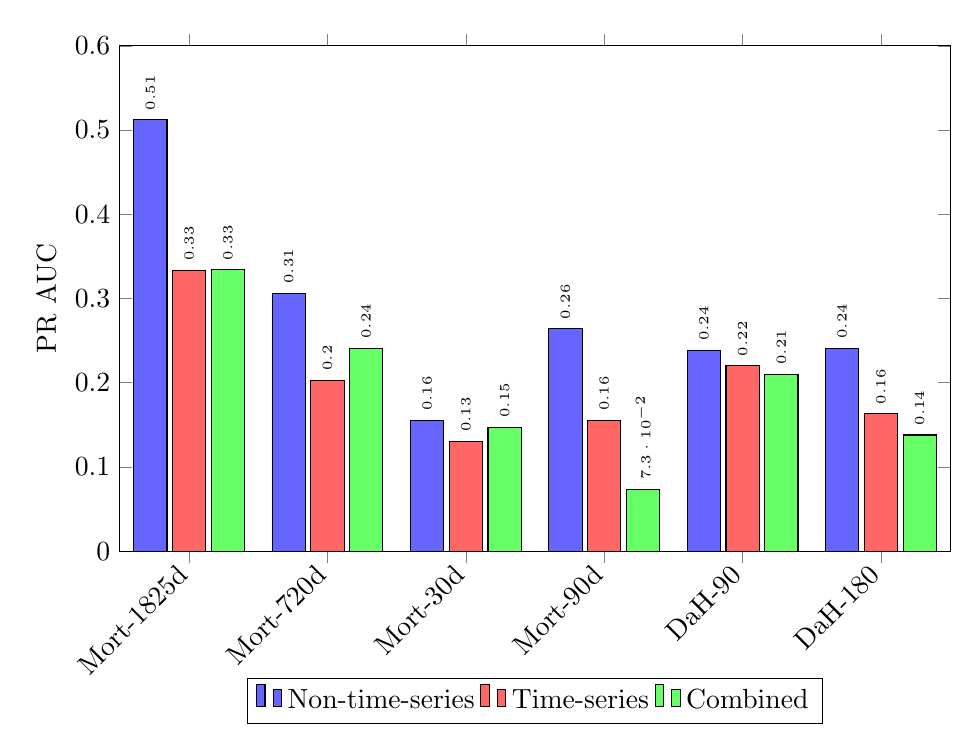
\begin{tikzpicture}
    \begin{axis}[
        width=\textwidth,
        height=8cm,
        ybar,
        bar width=12pt,
        ylabel={PR AUC},
        xlabel={Outcome},
        ymin=0,
        ymax=0.6,
        symbolic x coords={Mort-1825d, Mort-720d, Mort-30d, Mort-90d, DaH-90, DaH-180},
        xtick=data,
        xticklabel style={rotate=45,anchor=east},
        legend style={at={(0.5,-0.25)},anchor=north,legend columns=3},
        nodes near coords,
        nodes near coords style={font=\tiny},
        every node near coord/.append style={rotate=90,anchor=west}
    ]
    
    \addplot[fill=blue!60] coordinates {
        (Mort-1825d,0.512)
        (Mort-720d,0.306)
        (Mort-30d,0.155)
        (Mort-90d,0.264)
        (DaH-90,0.238)
        (DaH-180,0.241)
    };
    
    \addplot[fill=red!60] coordinates {
        (Mort-1825d,0.333)
        (Mort-720d,0.203)
        (Mort-30d,0.130)
        (Mort-90d,0.155)
        (DaH-90,0.220)
        (DaH-180,0.163)
    };
    
    \addplot[fill=green!60] coordinates {
        (Mort-1825d,0.334)
        (Mort-720d,0.241)
        (Mort-30d,0.147)
        (Mort-90d,0.073)
        (DaH-90,0.210)
        (DaH-180,0.138)
    };
    
    \legend{Non-time-series,Time-series,Combined}
    \end{axis}
    \end{tikzpicture}
\end{document}
